\documentclass[slides]{pgnotes}

\title{Practices}

\begin{document}

\maketitle

\tableofcontents

\section{Scenario}

\begin{center}
  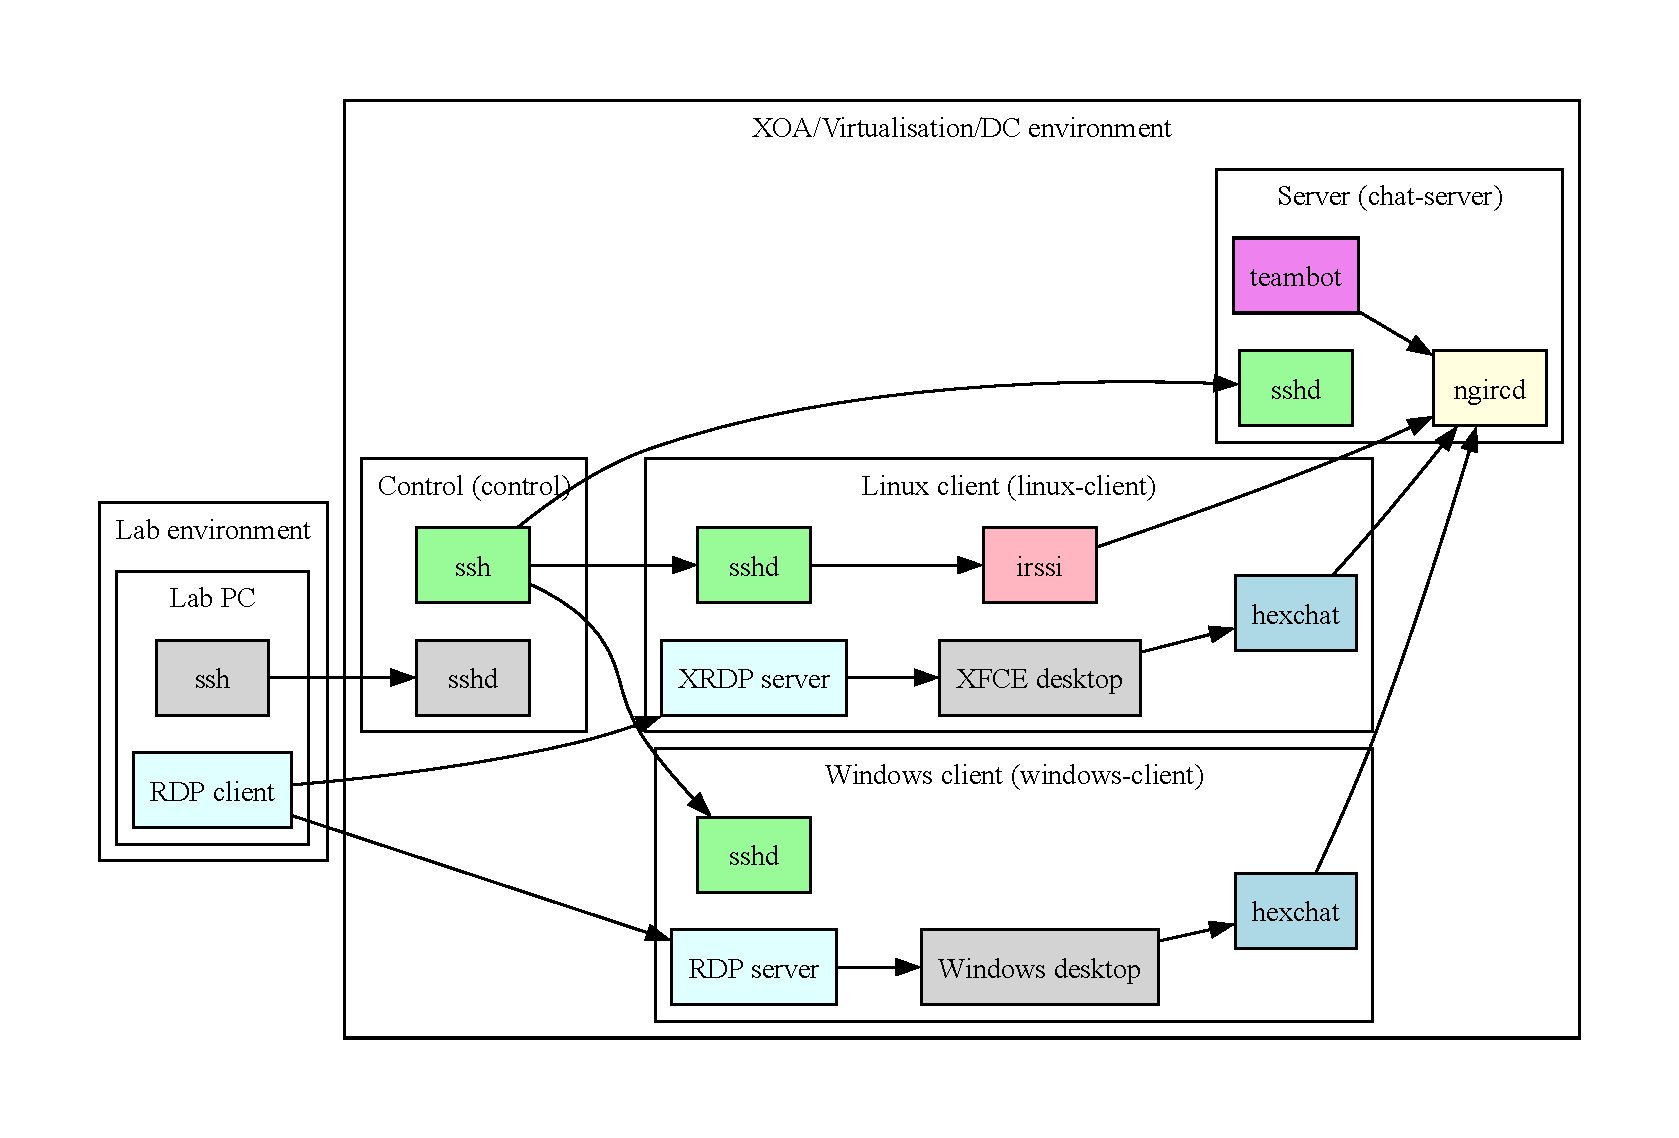
\includegraphics[width=0.7\linewidth]{scenario}
\end{center}

\section{Infrastructural practices}

\subsection{Addressing}

Your target nodes are inventoried as either IP addresses or hostnames.

Sometimes a playbook will reboot a host:
\begin{itemize}
\item Best to ensure that hosts always receive the same IP address.
\item DHCP reservation is better than a static address.
\item Dynamic DNS registration also a possibility (not for here!)
\end{itemize}

\begin{greenbox}{Ensure hosts receive same IP address}
  \begin{itemize}
  \item Hosts should have a DHCP reservation.
  \item Consider generating inventory file dynamically from DNS / DHCP files.
  \end{itemize}
\end{greenbox}

\subsection{Uniformity}

While ansible itself is cross-platform, its modules are not.

For example, in terms of package management:
\begin{itemize}
\item Debian and Ubuntu use \texttt{apt}
\item RedHat uses \texttt{yum}
\item Windows internally uses MSI files
\end{itemize}

As we have seen so far, the same operations on Windows and Linux are handled by different ansible modules.

\begin{greenbox}{Standardise where possible}
  \begin{itemize}
  \item When you have the opportunity to standardise your environment, take it!
  \end{itemize}
\end{greenbox}

\subsection{Hostnames}

We often use hostnames instead of IP addresses. 

Although the aim of automation is to reduce manual intervention, you can often find yourself logged in to multiple similar hosts:
\begin{itemize}
\item The only way to distingush them is by means of their displayed hostname.
\item This will only work if the hostname has been set.
\item Can happen during OS installation
\item Or can be set by DHCP client if received from DHCP server.
\end{itemize}

\begin{greenbox}{Set the hostname!}
  \begin{itemize}
  \item Manually using \texttt{hostnamectl}
  \item Or by \texttt{hostname} module in Ansible playbook
  \end{itemize}
\end{greenbox}



\section{Coding practices}

\subsection{Version control your code}

Your playbook(s) are living documents:
\begin{itemize}
\item You need to be able to experiment with changes.
\item Bugs / regressions can creep in when changes are made.
\item Requirements change over time.
\item Syntax and other mistakes can be amde.
\end{itemize}

\textbf{You need to be able to see changes between versions and roll back to previous versions.}

\begin{greenbox}{Use version control}
  \begin{itemize}
  \item Your playbooks should be kept in a version control system.
  \item Highly recommend \texttt{git} as used throughout industry.
  \end{itemize}
\end{greenbox}


\subsection{Editor}

Playbooks are written in YAML / YML syntax.

Don't even try to edit this in Word!

\begin{greenbox}{Use a suitable editor}
  \begin{itemize}
  \item At a minimum, use an editor that can syntax highlight YML.
  \item Better still if it can automate some YML formatting as well.
  \end{itemize}
\end{greenbox}

I use \texttt{emacs} with \texttt{yaml-mode} on both linux and windows.


\subsection{Check syntax}

Ansible has a \texttt{--check} option.

This depends on the implementation of the dry run / check operation in the modules used in the playbook.

Less useful if there are conditional / dependent operations in the playbook.


\section{Playbook practices}

\subsection{Handling reboots}

Reboots are sometimes required or recommended following certain system updates.

Ansible can initiate and wait for a reboot on a target node.

\begin{greenbox}{Smart reboots}
  \begin{itemize}
  \item Reboots should normally be conditional (if possible)
  \item Reboots won't work when running a playbook against the localhost
  \end{itemize}
\end{greenbox}


\subsection{Avoid shell commands}

On both Windows and Linux you can use Ansible to execute a shell command as if in a Bash / PowerShell script.

\begin{greenbox}{Use ansible native tasks}
  \begin{itemize}
  \item Replace any shell commands by ansible native tasks, where possible
  \end{itemize}
\end{greenbox}


\end{document}

